\chapter[Protótipos]{Protótipos}
\label{chap:prototipos}

	A seguir, são apresentados os prototipos idealizados a partir dos estudos efetuados durante o processo de estudo do problema.
	
	Serão descritos aqui protótipos de papel, protótipos de baixa fidelidade e de alta fidelidade, seguindo as fotografias das telas da respectiva solução de software. A proposta de solução como bem explicado nos capítulos anteriores trata-se de um \emph{app} (aplicativo móvel) para as plataformas Android, iOS e Windows Phone.

	\section[Protótipos de Papel]{Protótipos de Papel}
	\label{sec:prototipos_papel}

		A construção de protótipos em papel é uma técnica clássica de grande aceitação no meio dos especialistas em projetos de interfaces de usuário devido à sua simplicidade, ao seu baixo custo e por ser bastante efetiva. Ela consiste em esboçar telas e objetos de interação (de acordo com o projeto de interação proposto) em papéis no tamanho real esperado para cada um. Durante uma sessão de teste o esboço da janela principal é apresentado e é dada uma tarefa típica para ser executada pelo participante. Com um dedo o participante aponta e toca no esboço para indicar onde ele clicaria ou relata com que informação preencheria um particular campo de uma caixa de diálogo ou de um formulário eletrônico. \cite{paper}

		Abaixo são apresentadas as imagens dos protótipos de papel desenvolvidos para a aplicação.

		\newpage
		\begin{landscape}
		\begin{figure}[!htb]
			\centering
			\subfloat[Tela 1]{
				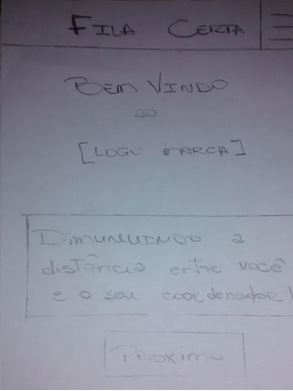
\includegraphics[width=5cm, height=7cm]{papel1}
				\label{papel1}
			}
			\quad %espaco separador
			\subfloat[Tela 2]{
				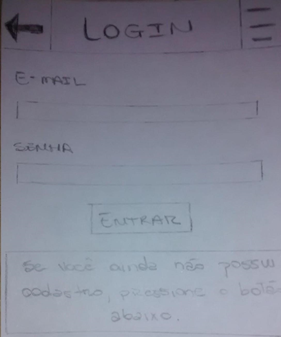
\includegraphics[width=5cm, height=7cm]{papel2}
				\label{papel2}
			}
			\quad
			\subfloat[Tela 3]{
				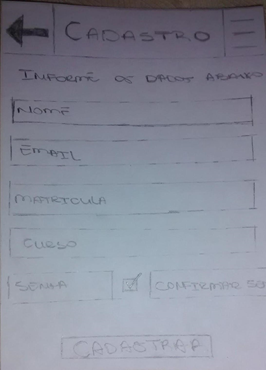
\includegraphics[width=5cm, height=7cm]{papel3}
				\label{papel3}
			}
			\quad
			\subfloat[Tela 4]{
				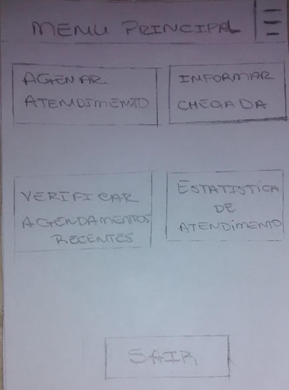
\includegraphics[width=5cm, height=7cm]{papel4}
				\label{papel4}
			}
			\quad
			\subfloat[Tela 5]{
				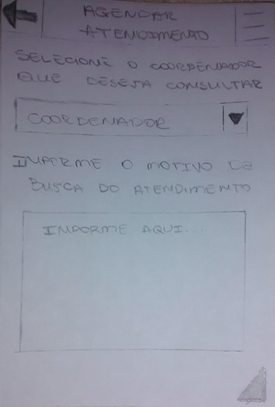
\includegraphics[width=5cm, height=7cm]{papel5}
				\label{papel5}
			}	
			\quad
			\subfloat[Tela 6]{
				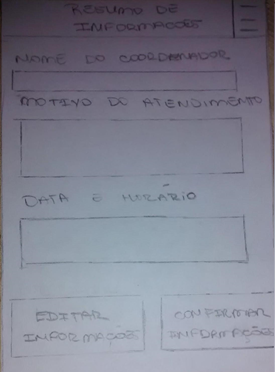
\includegraphics[width=5cm, height=7cm]{papel7}
				\label{papel6}
			}	
			\quad
			\subfloat[Tela 7]{
				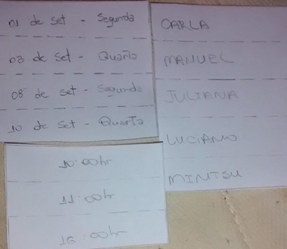
\includegraphics[width=8cm, height=7cm]{papel8}
				\label{papel7}
			}	
			\caption{Protótipos de Papel.}
			\label{fig01}
		\end{figure}
		\end{landscape}

	\section[Protótipos de Baixa Fidelidade]{Protótipos de Baixa Fidelidade}
	\label{sec:prototipos_baixa}

		Os protótipos de baixa fidelidade, também chamados de rascunhos ou sketches, são concebidos ainda na fase inicial, durante a concepção do sistema.
		
		Desenhados geralmente à mão utilizando lápis, borracha e papel, essas representações são feitas de maneira rápida e superficial, apenas margeando a ideia do projeto e definindo superficialmente sua interação com o usuário, não se preocupando ainda com elementos de layout, cores, disposições, etc.

		Essa etapa é fundamental para a definição do produto e levantamento de requisitos.

		Abaixo são apresentadas as imagens dos protótipos de baixa fidelidade desenvolvidos para a aplicação.

		\newpage
		\begin{landscape}
		\begin{figure}[!htb]
			\centering
			\subfloat[Tela 1]{
				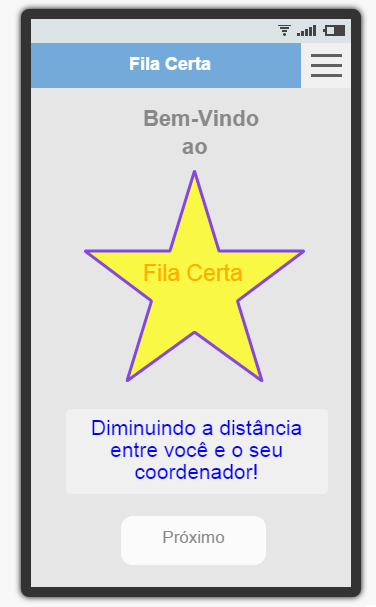
\includegraphics[width=5cm, height=7cm]{baixa1}
				\label{baixa1}
			}
			\quad %espaco separador
			\subfloat[Tela 2]{
				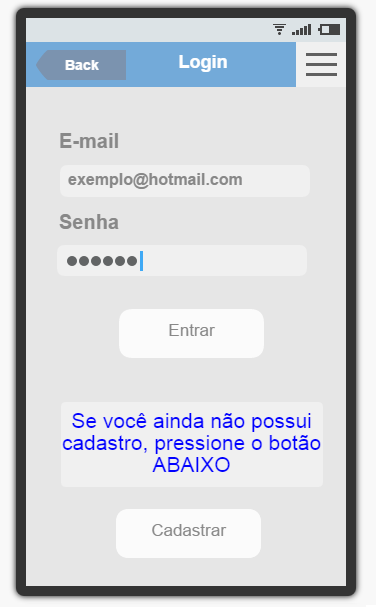
\includegraphics[width=5cm, height=7cm]{baixa2}
				\label{baixa2}
			}
			\quad
			\subfloat[Tela 3]{
				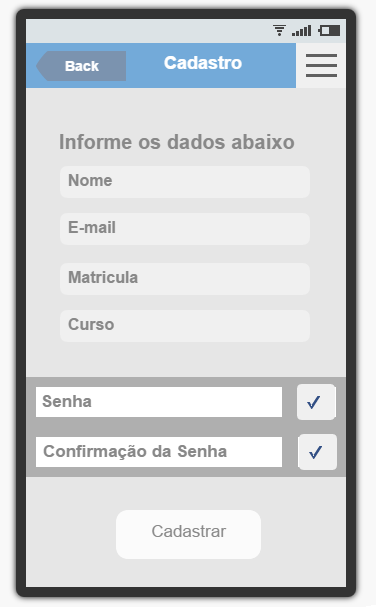
\includegraphics[width=5cm, height=7cm]{baixa3}
				\label{baixa3}
			}
			\quad
			\subfloat[Tela 4]{
				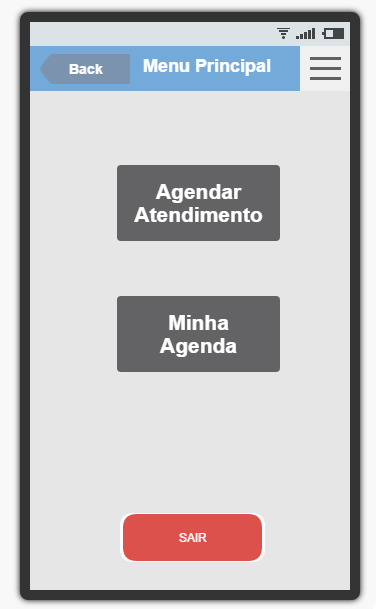
\includegraphics[width=5cm, height=7cm]{baixa4}
				\label{baixa4}
			}
			\quad
			\subfloat[Tela 5]{
				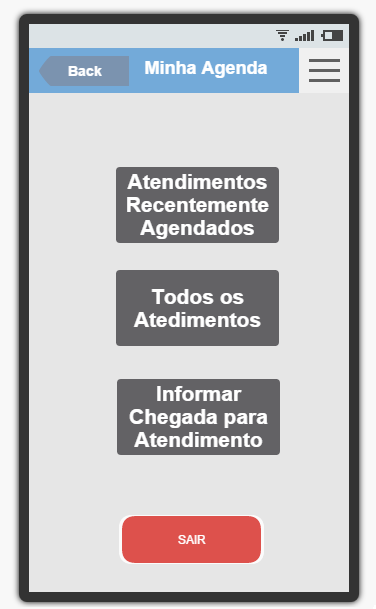
\includegraphics[width=4.3cm, height=7cm]{baixa5}
				\label{baixa5}
			}	
			\quad
			\subfloat[Tela 6]{
				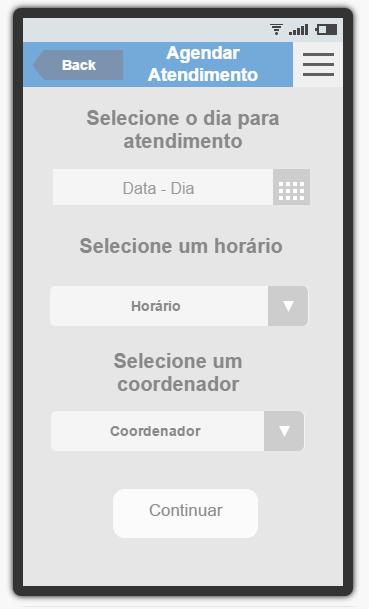
\includegraphics[width=4.3cm, height=7cm]{baixa6}
				\label{baixa6}
			}	
			\quad
			\subfloat[Tela 7]{
				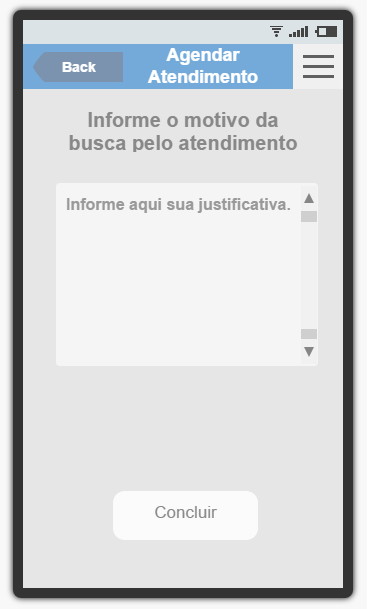
\includegraphics[width=4.3cm, height=7cm]{baixa7}
				\label{baixa7}
			}
			\quad
			\subfloat[Tela 8]{
				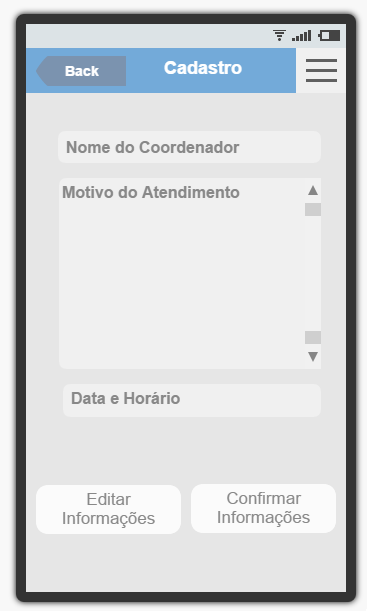
\includegraphics[width=4.3cm, height=7cm]{baixa8}
				\label{baixa8}
			}
			\quad
			\subfloat[Tela 9]{
				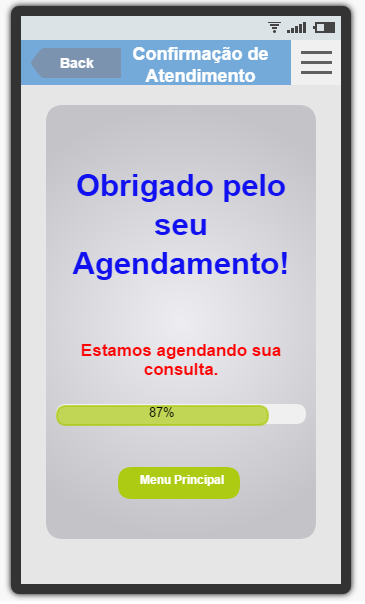
\includegraphics[width=4.3cm, height=7cm]{baixa9}
				\label{baixa9}
			}
			\caption{Protótipos de Baixa Fidelidade.}
			\label{fig02}
		\end{figure}
		\end{landscape}


	\section[Protótipos de Alta Fidelidade]{Protótipos de Alta Fidelidade}
	\label{sec:prototipos_alta}

		Os mockups ou protótipos funcionais constituem a representação mais próxima do sistema a ser desenvolvido. Em alguns casos, é possível simular o fluxo completo das funcionalidades, permitindo a interação do usuário como se fosse o produto final.

		A aparência visual, as formas de navegação e interatividade já são concebidas e aplicadas aos protótipos de alta fidelidade.

		Seu desenvolvimento é realizado na fase final de definição da interface, utilizando programas de design gráfico, como o Photoshop ou Fireworks; ferramentas de codificação front-end, como o Sublime Text ou Dreamweaver; e linguagens de programação front-end, como o HTML + CSS + jQuery. \cite{alta}

		Abaixo são apresentadas as imagens dos protótipos de alta fidelidade desenvolvidos para a aplicação tanto para primeira interação quanto para segunda.

		\newpage
		\begin{landscape}
		\subsection[Primeira Interação]{Primeira Interação}
		\label{sec:prototipos_alta_1}
			
			\begin{figure}[!htb]
				\centering
				\subfloat[Tela 1]{
					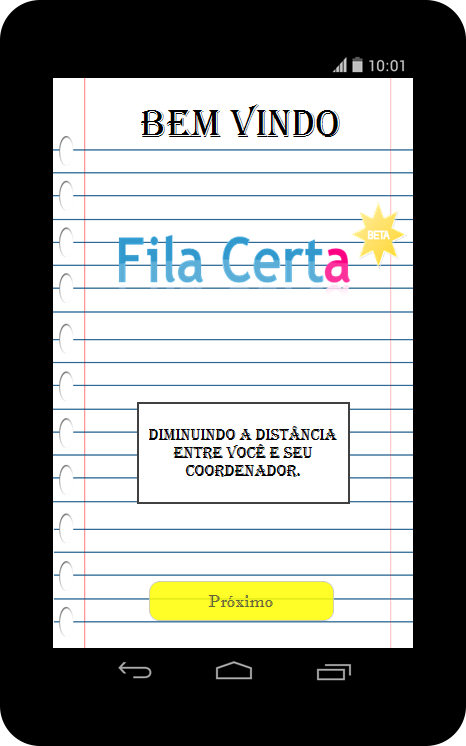
\includegraphics[width=5cm, height=8cm]{parteI}
					\label{alta1}
				}
				\quad %espaco separador
				\subfloat[Tela 2]{
					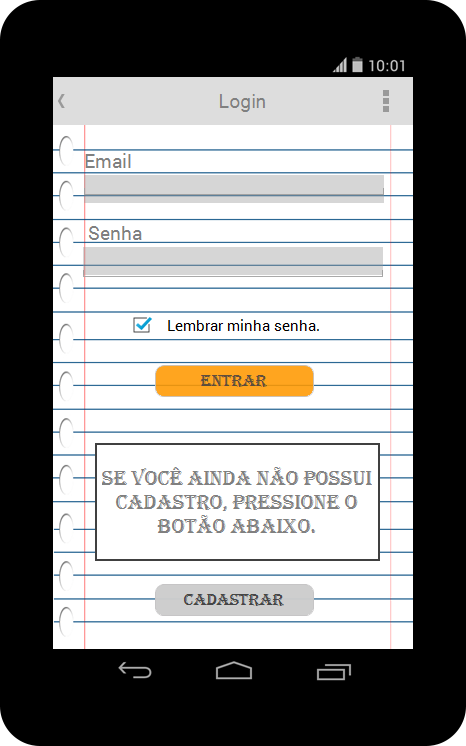
\includegraphics[width=5cm, height=8cm]{parteII}
					\label{alta2}
				}
				\quad
				\subfloat[Tela 3]{
					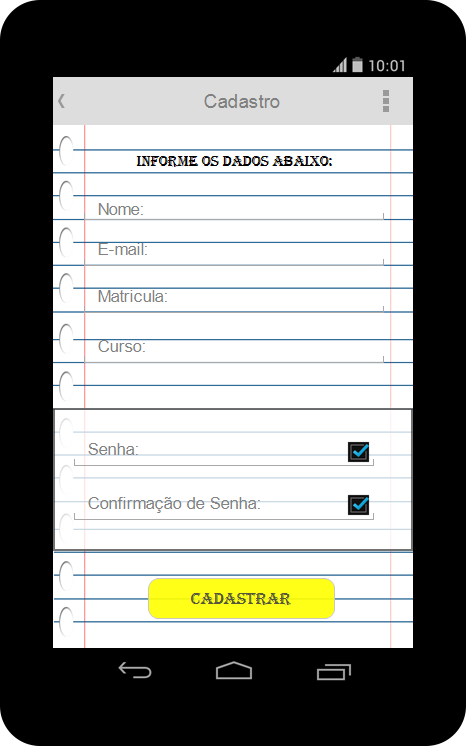
\includegraphics[width=5cm, height=8cm]{parteIII}
					\label{alta3}
				}
				\quad
				\subfloat[Tela 4]{
					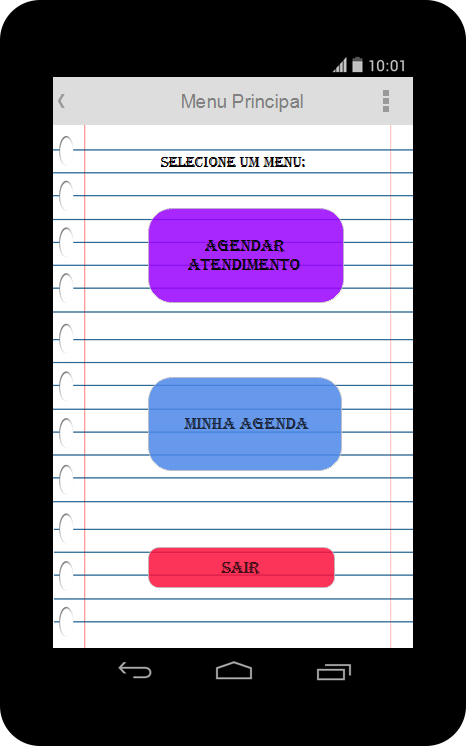
\includegraphics[width=5cm, height=8cm]{parteIV}
					\label{alta4}
				}
				\caption[Protótipos de Alta Fidelidade - Parte I]{Protótipos de Alta Fidelidade - Parte I.}
				\label{fig03-1int}
			\end{figure}

			\begin{figure}[!htb]
				\centering
				\subfloat[Tela 5]{
					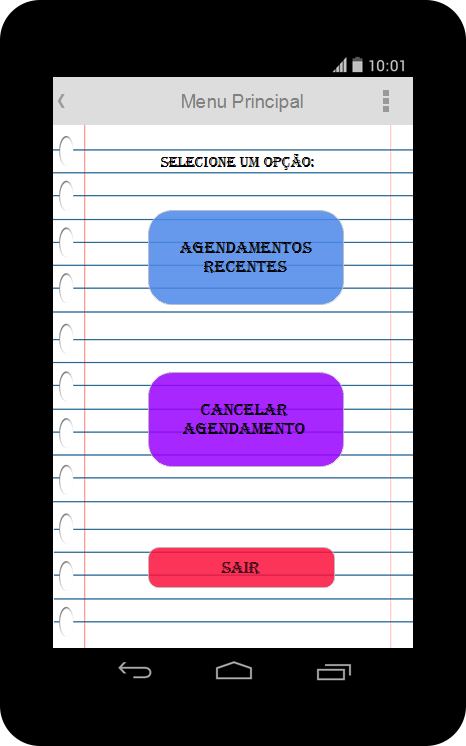
\includegraphics[width=5cm, height=7cm]{parteV}
					\label{alta5}
				}	
				\quad
				\subfloat[Tela 6]{
					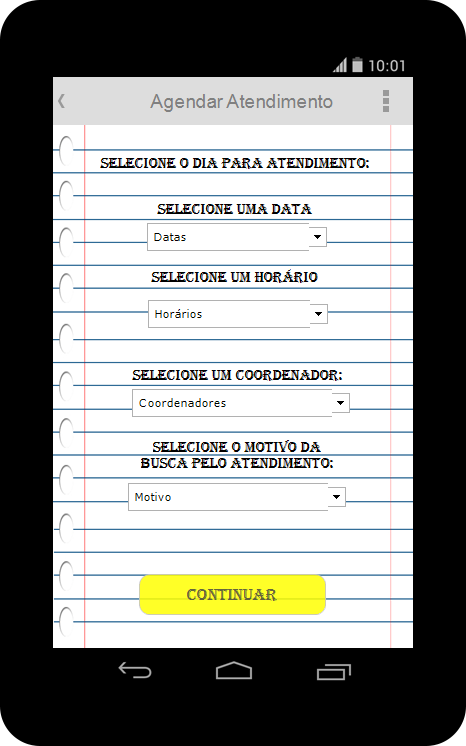
\includegraphics[width=5cm, height=7cm]{parteVI}
					\label{alta6}
				}	
				\quad
				\subfloat[Tela 7]{
					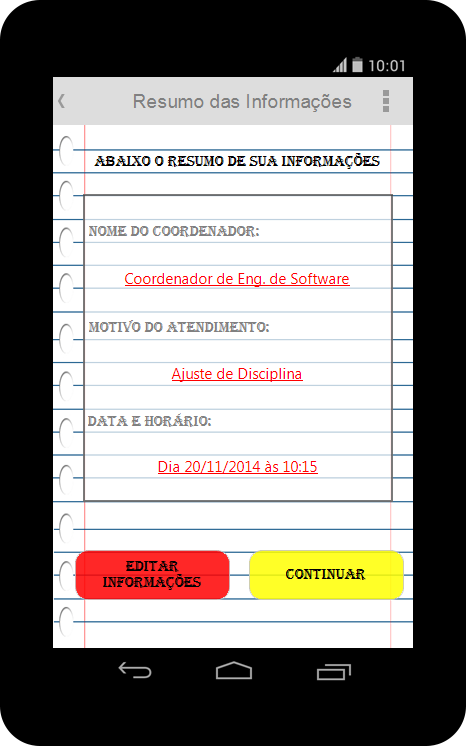
\includegraphics[width=5cm, height=7cm]{parteVII}
					\label{alta7}
				}
				\quad
				\subfloat[Tela 8]{
					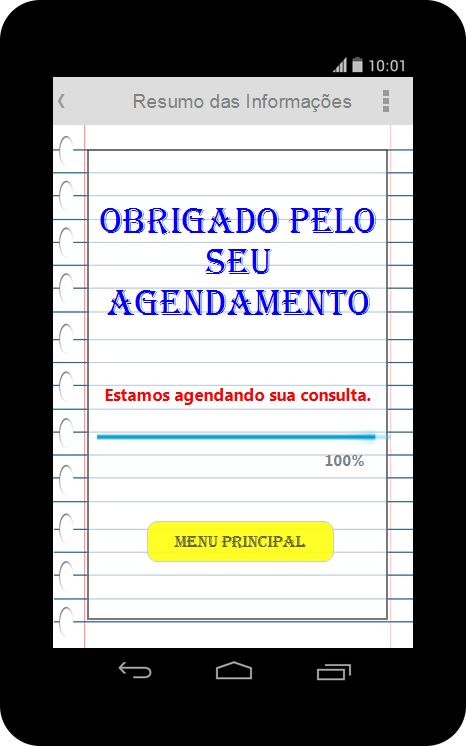
\includegraphics[width=5cm, height=7cm]{parteVIII}
					\label{alta8}
				}			
				\quad
				\subfloat[Tela 9]{
					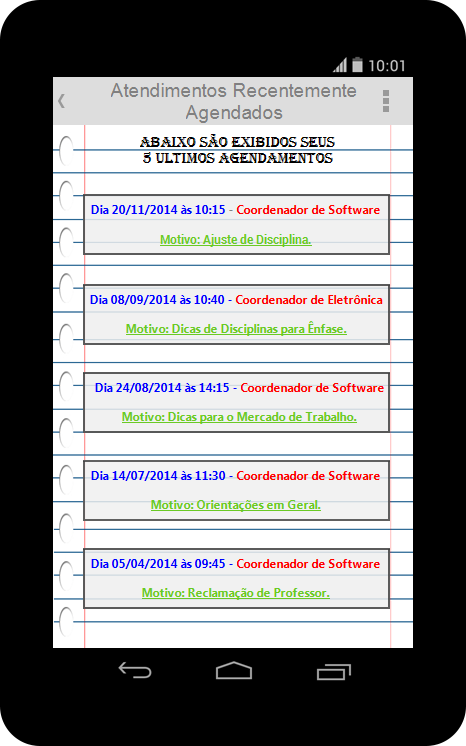
\includegraphics[width=5cm, height=7cm]{parteIX}
					\label{alta9}
				}
				\quad
				\subfloat[Tela 10]{
					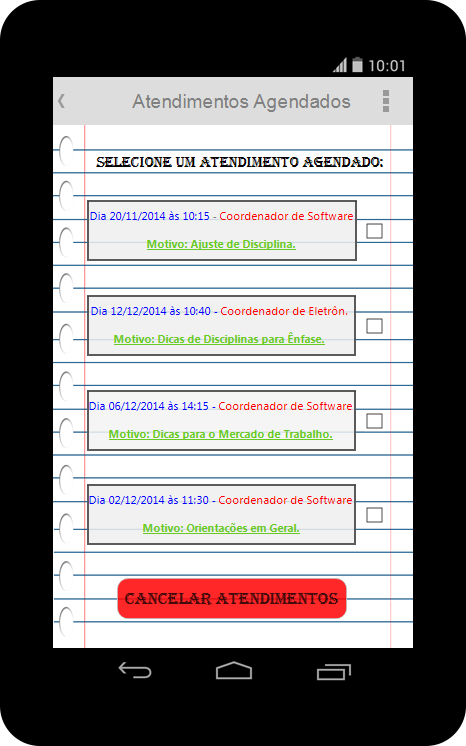
\includegraphics[width=5cm, height=7cm]{parteX}
					\label{alta10}
				}
				\quad
				\subfloat[Tela 11]{
					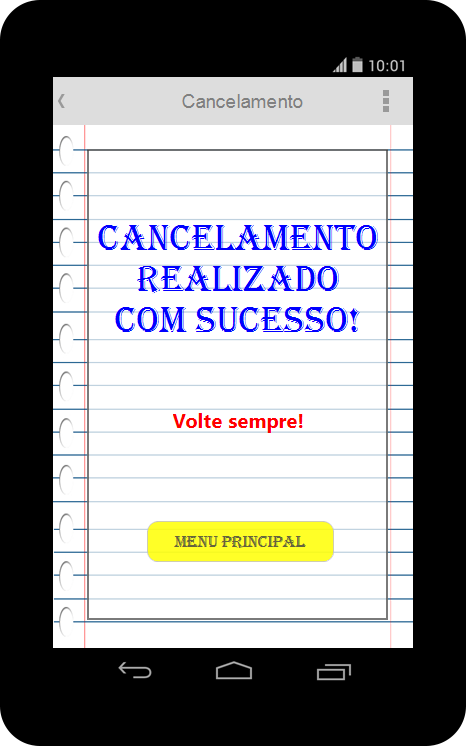
\includegraphics[width=5cm, height=7cm]{parteXI}
					\label{alta11}
				}
				\caption[Protótipos de Alta Fidelidade - Parte II]{Protótipos de Alta Fidelidade - Parte II.}
				\label{fig03-1int}
			\end{figure}
		\end{landscape}

			\begin{figure}[!htb]
				\centering
				\subfloat[Mapa de Navegação]{
					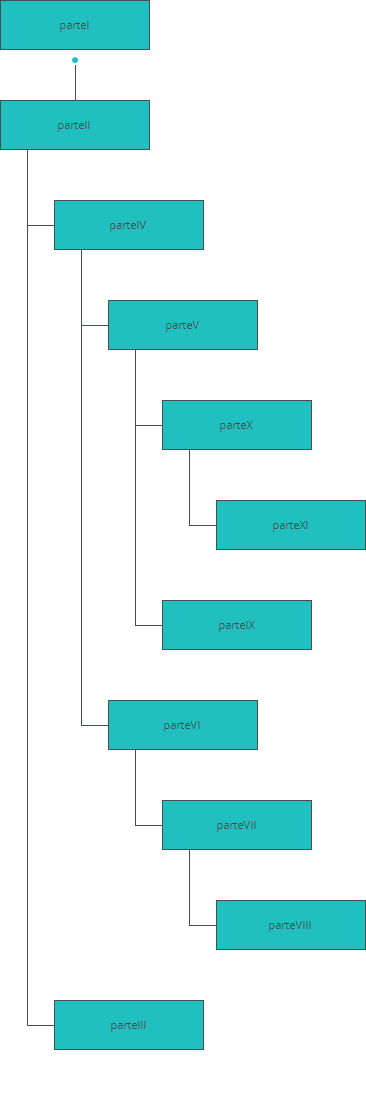
\includegraphics[width=10cm, height=22cm]{mapa}
					\label{mapaInt1}
				}
				\caption[Protótipos de Alta Fidelidade - Parte III]{Protótipos de Alta Fidelidade - Parte III.}
				\label{fig03-1int}
			\end{figure}
		

		\newpage
		\begin{landscape}
		\subsection[Segunda Interação]{Segunda Interação}
		\label{sec:prototipos_alta_2}
			
			\begin{figure}[!htb]
				\centering
				\subfloat[Tela 1]{
					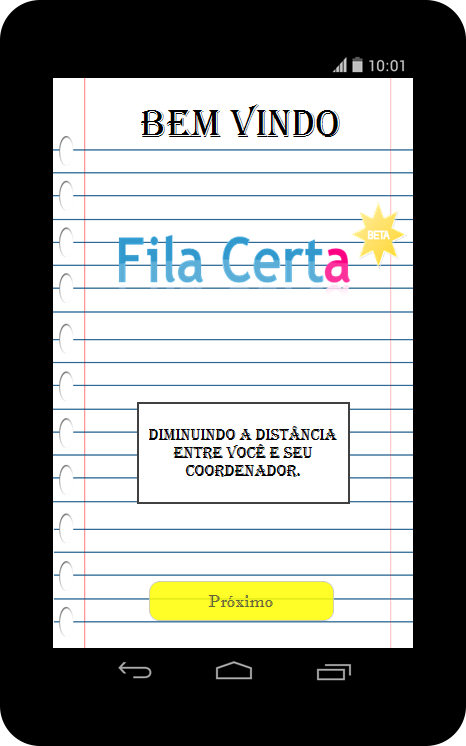
\includegraphics[width=5cm, height=8cm]{parteI}
					\label{alta1}
				}
				\quad %espaco separador
				\subfloat[Tela 2]{
					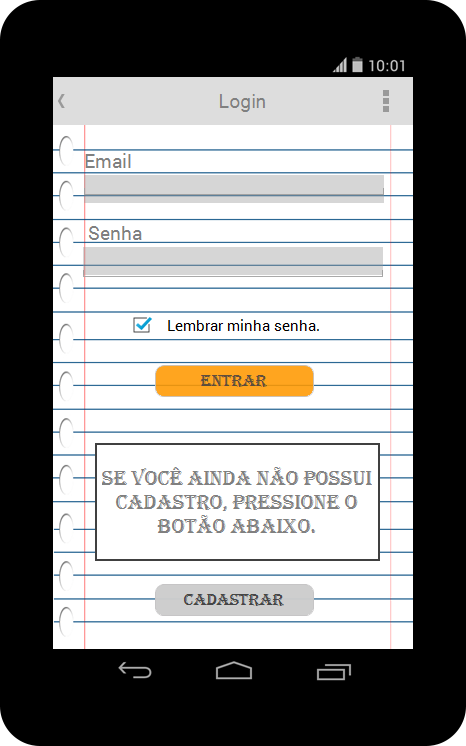
\includegraphics[width=5cm, height=8cm]{parteII}
					\label{alta2}
				}
				\quad
				\subfloat[Tela 3]{
					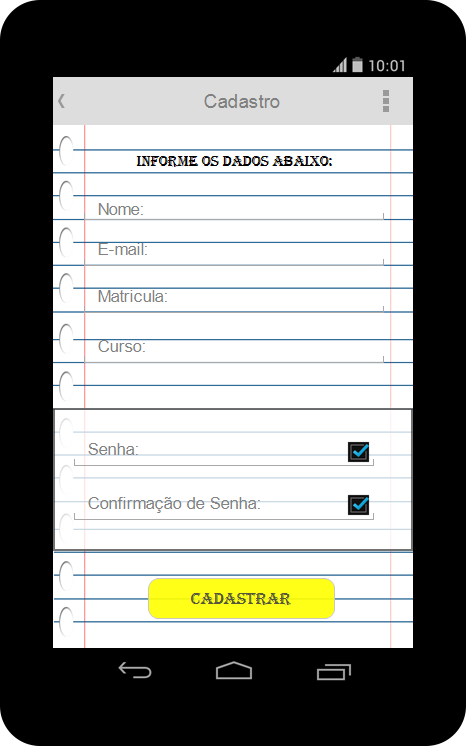
\includegraphics[width=5cm, height=8cm]{parteIII}
					\label{alta3}
				}
				\quad
				\subfloat[Tela 4]{
					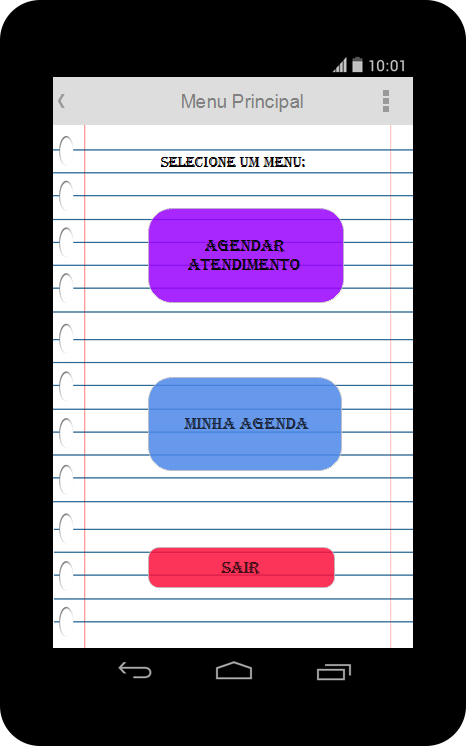
\includegraphics[width=5cm, height=8cm]{parteIV}
					\label{alta4}
				}
				\caption[Protótipos de Alta Fidelidade - Parte I]{Protótipos de Alta Fidelidade - Parte I.}
				\label{fig03-1int}
			\end{figure}

			\begin{figure}[!htb]
				\centering
				\subfloat[Tela 5]{
					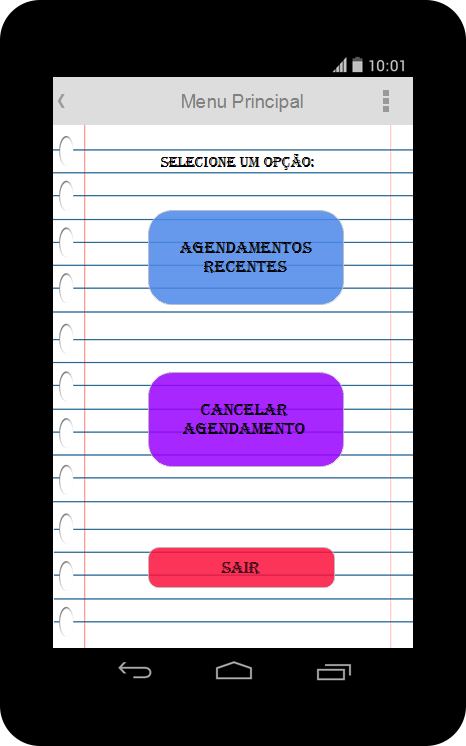
\includegraphics[width=5cm, height=7cm]{parteV}
					\label{alta5}
				}	
				\quad
				\subfloat[Tela 6]{
					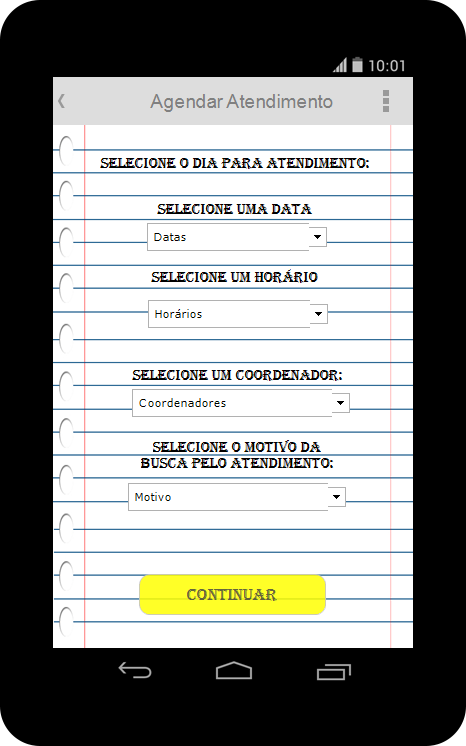
\includegraphics[width=5cm, height=7cm]{parteVI}
					\label{alta6}
				}	
				\quad
				\subfloat[Tela 7]{
					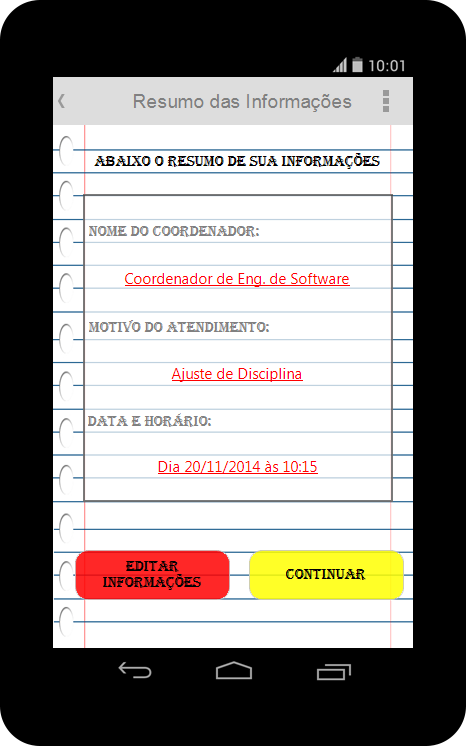
\includegraphics[width=5cm, height=7cm]{parteVII}
					\label{alta7}
				}
				\quad
				\subfloat[Tela 8]{
					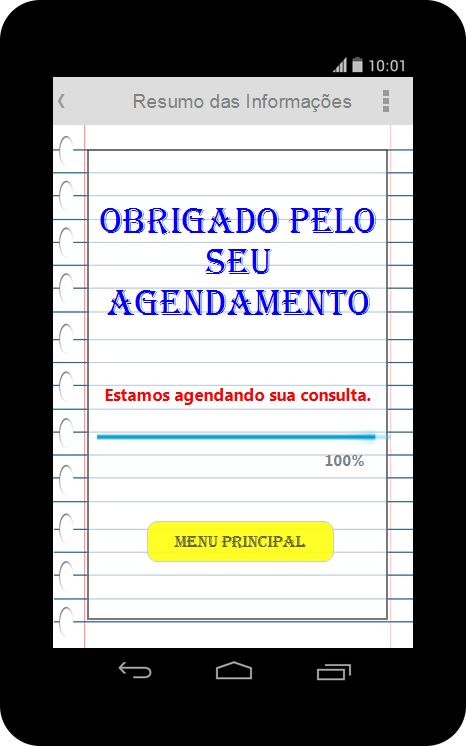
\includegraphics[width=5cm, height=7cm]{parteVIII}
					\label{alta8}
				}			
				\quad
				\subfloat[Tela 9]{
					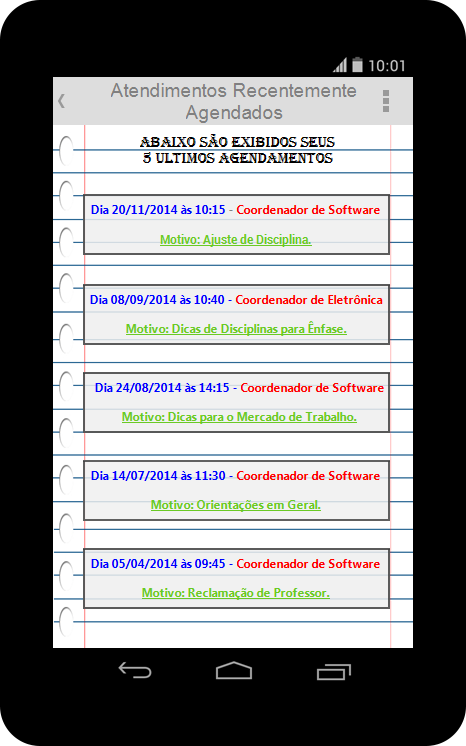
\includegraphics[width=5cm, height=7cm]{parteIX}
					\label{alta9}
				}
				\quad
				\subfloat[Tela 10]{
					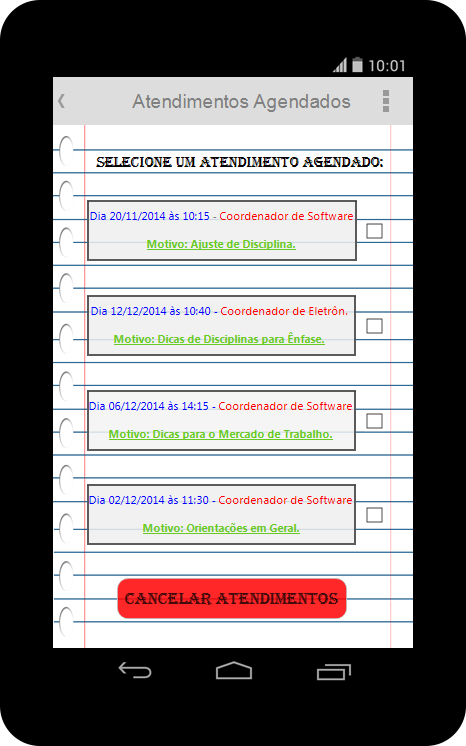
\includegraphics[width=5cm, height=7cm]{parteX}
					\label{alta10}
				}
				\quad
				\subfloat[Tela 11]{
					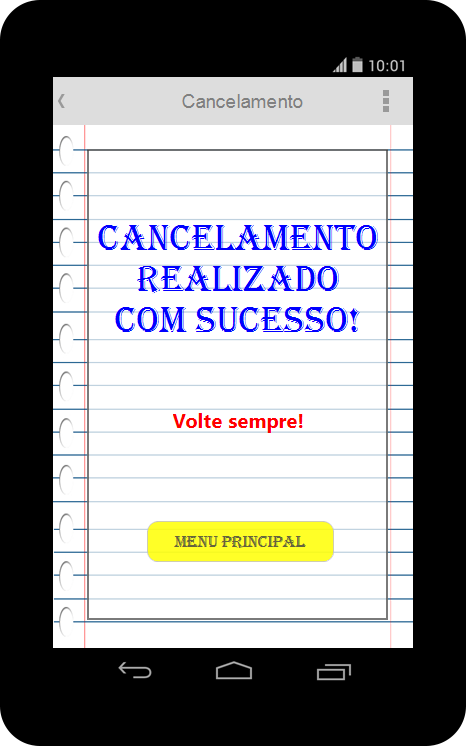
\includegraphics[width=5cm, height=7cm]{parteXI}
					\label{alta11}
				}
				\caption[Protótipos de Alta Fidelidade - Parte II]{Protótipos de Alta Fidelidade - Parte II.}
				\label{fig03-1int}
			\end{figure}
		\end{landscape}

			\begin{figure}[!htb]
				\centering
				\subfloat[Mapa de Navegação]{
					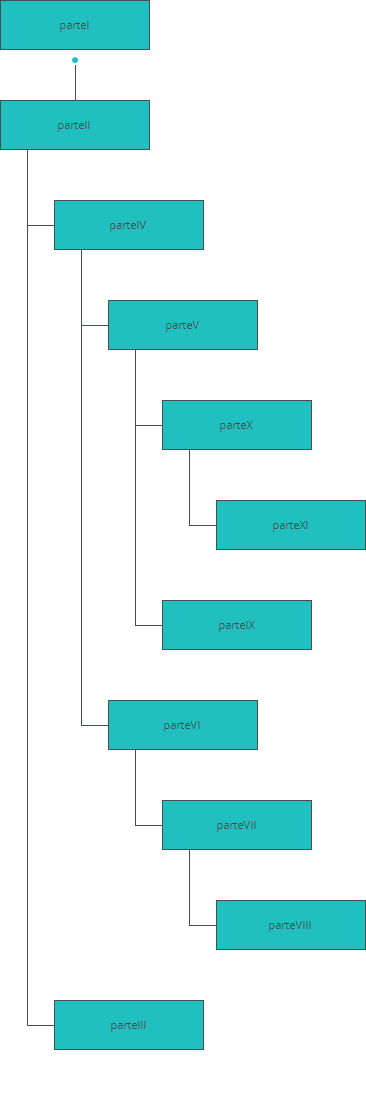
\includegraphics[width=10cm, height=22cm]{mapa}
					\label{mapaInt1}
				}
				\caption[Protótipos de Alta Fidelidade - Parte III]{Protótipos de Alta Fidelidade - Parte III.}
				\label{fig03-1int}
			\end{figure}